\documentclass[11pt,letterpaper]{article}
\usepackage[utf8]{inputenc}

%----- Configuración del estilo del documento------%
\usepackage[table]{xcolor}
\usepackage{epsfig,graphicx}
\usepackage[left=2cm,right=2cm,top=1.8cm,bottom=2.3cm]{geometry}
\usepackage{fancyhdr}
\usepackage{lastpage}

\fancyhf{}
\rfoot{\textit{Página \thepage \hspace{1pt} de \pageref{LastPage}}}


%------ Paquetes matemáticos básicos --------%
\usepackage{amsmath}
\usepackage{amsfonts}
\usepackage{amssymb}
\usepackage{amsthm}
\usepackage{geometry}
\geometry{margin=1in}

%------ Texto aleatorio ----- %

\usepackage{lipsum}
\usepackage{enumitem}



\begin{document}

%------ Encabezado -------- %

\begin{center}
    \begin{minipage}{3cm}
    	\begin{center}
    		\includegraphics[height=3.4cm]{./imagenes/logo_unam.png}
    	\end{center}
    \end{minipage}\hfill
    \begin{minipage}{10cm}
    	\begin{center}
    	\textbf{\large Universidad Nacional Autónoma de México}\\[0.1cm]
        \textbf{Facultad de Ciencias}\\[0.1cm]
        \textbf{Matemáticas para las Ciencias Aplicadas $|$ Grupo 7048}\\[0.1cm]
        \textbf{Tarea 4 }\\[0.1cm]
        Real Araiza Yamile\\[0.1cm]
        Rodríguez López Luis Fernando\\[0.1cm]
        Tenorio Reyes Ihebel Luro\\[0.1cm]
        25/11/2024
    	\end{center}
    \end{minipage}\hfill
    \begin{minipage}{3cm}
    	\begin{center}
    		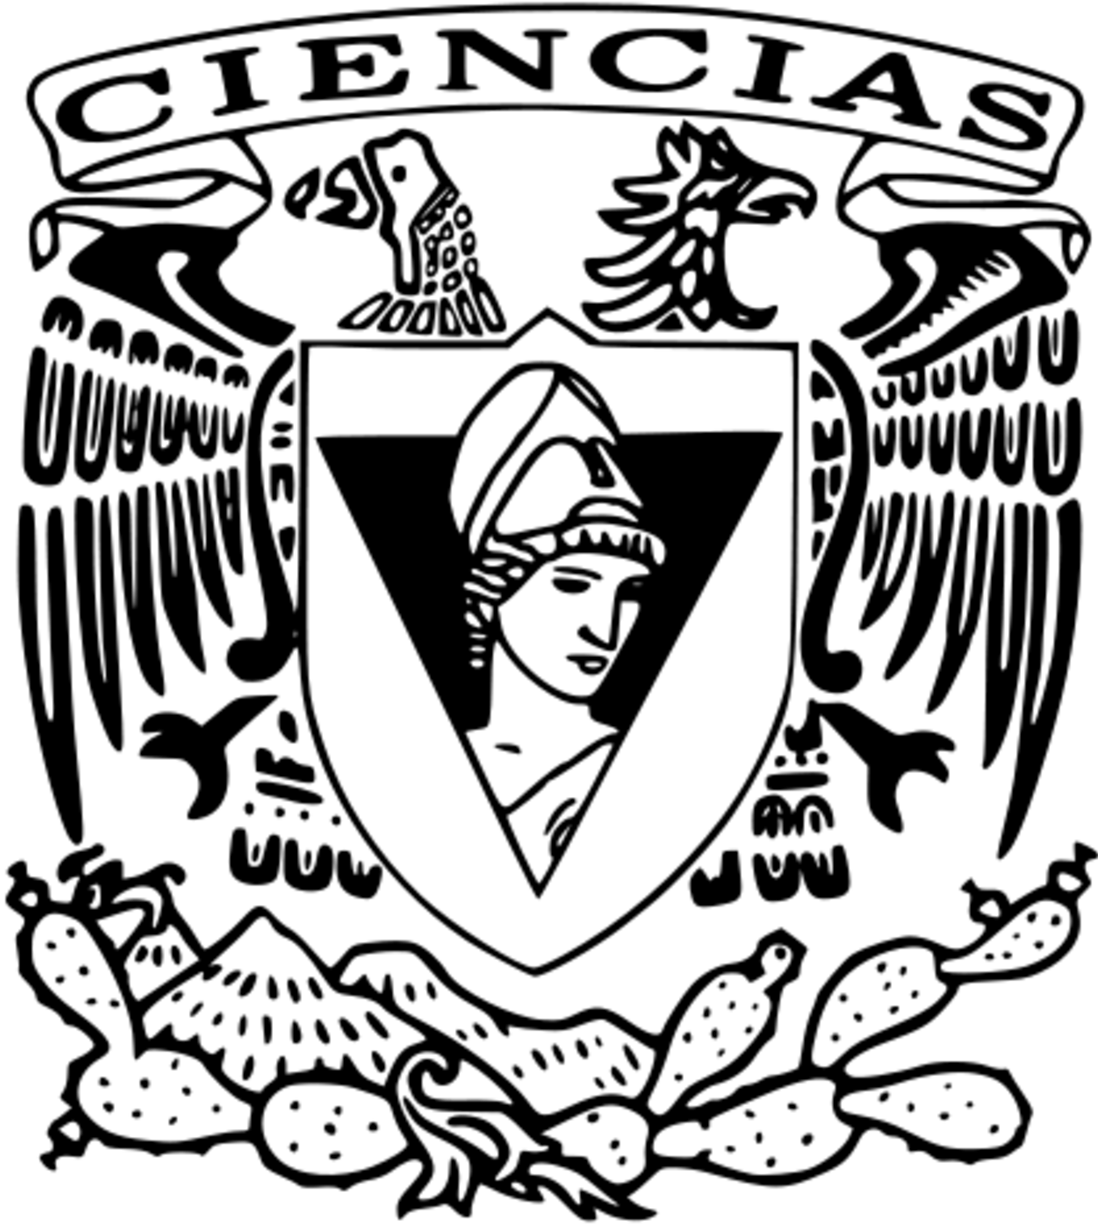
\includegraphics[height=3.4cm]{./imagenes/Logo_FC.png}
    	\end{center}
    \end{minipage}
\end{center}

\rule{17cm}{0.1mm}

%------ Fin de encabezado -------- %

%\section*{1ra Parte}

\subparagraph{Ejercicios: Review Exercises Capítulo 5 Anton-Bivens-Davis (pp. 408-412).}

% ---- 01. Ejercicio 13 IHEBEL ---- %
\section{Ejercicio 13, cap V Review Exercises.}
Evaluar la integral sustiyuyendo $u=x^2-1$
\begin{equation*}
  \int \frac{x}{(x^2-1)\sqrt{x^4-2x^2}}dx
\end{equation*}
Considerando:
\begin{equation*}
  \begin{split}
    u &= x^2-1\\
    u^2 &= x^4-2x^2+1\\
    du &= 2xdx\\
    dx &= \frac{du}{2x}
  \end{split}
\end{equation*}
Sustituyendo
\begin{equation*}
  \begin{split}
    \int \frac{x}{ (x^2-1) \sqrt{x^4-2x^2}} dx &= \int \frac{x\, du}{2x u \sqrt{u^2-1}} \\
    &= \frac{1}{2}\int \frac{du}{u\sqrt{u^2-1}} \\
    &= \frac{1}{2} \operatorname{sec}^{-1}\left(\frac{u}{1}\right) \quad \text{por fórmula 18} \\
    &= \frac{\operatorname{sec}^{-1}(u)}{2} \\
    &= \frac{\operatorname{arcsec}(x^2-1)}{2} + c
  \end{split}
\end{equation*}

% ---- 02. Ejercicio 23 YAMILE ---- %
\section{Ejercicio 23, cap V Review Exercises.}
\section*{Cálculo de aproximaciones al área bajo la curva \(y = \ln(x)\)}

Queremos calcular las aproximaciones con los puntos extremos izquierdo, derecho y puntos medios para estimar el área bajo la curva \(y = \ln(x)\) en el intervalo \([1, 2]\) utilizando \(n = 10\) subintervalos.

\subsection*{Paso 1: Determinar el ancho de los subintervalos}
\[
\Delta x = \frac{b - a}{n} = \frac{2 - 1}{10} = 0.1
\]

\subsection*{Paso 2: Determinar los puntos de los subintervalos}
Los puntos que dividen el intervalo \([1, 2]\) en 10 subintervalos son:
\[
x_0 = 1, \, x_1 = 1.1, \, x_2 = 1.2, \dots, x_{10} = 2
\]

\subsection*{Paso 3: Aproximaciones}

\subsubsection*{(a) Aproximación con puntos extremos izquierdos}
Usamos los puntos \(x_0, x_1, \dots, x_9\). La fórmula es:
\[
A_{\text{izq}} = \Delta x \sum_{i=0}^{n-1} f(x_i)
\]
Sustituyendo:
\[
A_{\text{izq}} = 0.1 \left[ \ln(1) + \ln(1.1) + \ln(1.2) + \cdots + \ln(1.9) \right]
\]
Evaluando \(f(x_i) = \ln(x_i)\):
\[
f(x_0) = \ln(1) = 0, \quad f(x_1) = \ln(1.1) \approx 0.0953, \quad f(x_2) = \ln(1.2) \approx 0.1823, \dots, f(x_9) = \ln(1.9) \approx 0.6419
\]
Sumamos los valores:
\[
\sum f(x_i) = 0 + 0.0953 + 0.1823 + 0.2624 + 0.3365 + 0.4055 + 0.4700 + 0.5306 + 0.5878 + 0.6419 = 3.5122
\]
Entonces:
\[
A_{\text{izq}} = 0.1 \cdot 3.5122 = 0.3512
\]

\subsubsection*{(b) Aproximación con puntos extremos derechos}
Usamos los puntos \(x_1, x_2, \dots, x_{10}\). La fórmula es:
\[
A_{\text{der}} = \Delta x \sum_{i=1}^{n} f(x_i)
\]
Sustituyendo:
\[
A_{\text{der}} = 0.1 \left[ \ln(1.1) + \ln(1.2) + \ln(1.3) + \cdots + \ln(2) \right]
\]
Evaluando \(f(x_i) = \ln(x_i)\):
\[
f(x_1) = \ln(1.1) \approx 0.0953, \quad f(x_2) = \ln(1.2) \approx 0.1823, \, \dots, \, f(x_{10}) = \ln(2) \approx 0.6931
\]
Sumamos los valores:
\[
\sum f(x_i) = 0.0953 + 0.1823 + 0.2624 + 0.3365 + 0.4055 + 0.4700 + 0.5306 + 0.5878 + 0.6419 + 0.6931 = 4.2054
\]
Entonces:
\[
A_{\text{der}} = 0.1 \cdot 4.2054 = 0.4205
\]

\subsubsection*{(c) Aproximación con puntos medios}
Usamos los puntos medios de cada subintervalo. La fórmula es:
\[
A_{\text{medio}} = \Delta x \sum_{i=1}^{n} f\left(\frac{x_{i-1} + x_i}{2}\right)
\]
Cálculo de los puntos medios:
\[
x_{\text{medio},1} = \frac{1 + 1.1}{2} = 1.05, \, x_{\text{medio},2} = \frac{1.1 + 1.2}{2} = 1.15, \dots, x_{\text{medio},10} = \frac{1.9 + 2}{2} = 1.95
\]
Evaluando \(f(x)\) en estos puntos medios:
\[
f(1.05) \approx 0.0488, \, f(1.15) \approx 0.1398, \dots, f(1.95) \approx 0.6678
\]
Sumamos los valores:
\[
\sum f(x_{\text{medio}}) = 0.0488 + 0.1398 + 0.2231 + 0.3001 + 0.3716 + 0.4383 + 0.5008 + 0.5593 + 0.6145 + 0.6678 = 3.8650
\]
Entonces:
\[
A_{\text{medio}} = 0.1 \cdot 3.8650 = 0.3865
\]

\subsection*{Resumen de Resultados}
\[
A_{\text{izq}} = 0.3512, \quad A_{\text{der}} = 0.4205, \quad A_{\text{medio}} = 0.3865
\]


% ---- 03. Ejercicio 42 YAMILE ---- %
\section{Ejercicio 42, cap V Review Exercises.}
\section*{Cálculo del área bajo la curva}

Queremos calcular el área bajo la curva \(f(x) = \frac{1}{x}\) en el intervalo \([1, e^3]\). Esto se realiza resolviendo la integral definida:

\[
\int_{1}^{e^3} \frac{1}{x} \, dx
\]

\subsection*{Paso 1: Resolver la integral indefinida}
Sabemos que:
\[
\int \frac{1}{x} \, dx = \ln|x| + C
\]

Por lo tanto, la integral definida es:
\[
\int_{1}^{e^3} \frac{1}{x} \, dx = \ln(x) \Big|_{1}^{e^3}
\]

\subsection*{Paso 2: Evaluar los límites}
Evaluamos los límites de integración:
\[
\ln(e^3) - \ln(1)
\]

Sabemos que:
\[
\ln(e^3) = 3 \quad \text{y} \quad \ln(1) = 0
\]

Por lo tanto:
\[
\ln(e^3) - \ln(1) = 3 - 0 = 3
\]

\subsection*{Resultado final}
El área bajo la curva \(f(x) = \frac{1}{x}\) en el intervalo \([1, e^3]\) es:
\[
\boxed{3}
\]


% ---- 04. Ejercicio 53 LUIS ---- %
\section{Ejercicio 53, cap V Review Exercises.}
\paragraph*{Usa la Parte 2 del Teorema Fundamental del Cálculo y (cuando sea necesario) la Fórmula (18) de la Sección 5.10 para encontrar la derivada.}
\begin{equation*}
  \frac{d}{dx}\left[\int_{2}^{\sin x} \frac{1}{1+t^3}dt\right]
  \vspace{0.3cm}
\end{equation*}

Utilizaremos la Fórmula (18) del texto, que establece:
\[
\frac{d}{dx}\left[\int_{a}^{g(x)} f(t) dt\right] = f(g(x))g'(x)
\]

Donde:
\begin{itemize}
    \item $f(g(x))$ significa evaluar el integrando en el límite superior
    \item $g'(x)$ es la derivada del límite superior
\end{itemize}

\subsection*{Desarrollo}
\begin{enumerate}
    \item Evaluamos $f(g(x))$:
    \[
    f(g(x)) = f(\sin x) = \frac{1}{1+(\sin x)^3}
    \]
    
    \item Calculamos $g'(x)$:
    \[
    g'(x) = \frac{d}{dx}(\sin x) = \cos x
    \]
    
    \item Aplicamos la fórmula:
    \[
    \frac{d}{dx}\left[\int_{2}^{\sin x} \frac{1}{1+t^3} dt\right] = \frac{1}{1+(\sin x)^3} \cdot \cos x
    \]
\end{enumerate}

\subsection*{Resultado}
\[
\boxed{\frac{d}{dx}\left[\int_{2}^{\sin x} \frac{1}{1+t^3} dt\right] = \frac{\cos x}{1+(\sin x)^3}}
\]



% ---- 05. Ejercicio 56 LUIS ---- %
\section{Ejercicio 56, cap V Review Exercises.}
\paragraph*{Dada la función \( F(x) = \int_0^x \frac{t^2 - 3}{t^4 + 7} \, dt \):}
\\
\begin{enumerate}
    \item[(a)] Encuentra los intervalos en los que \( F \) es creciente y aquellos en los que \( F \) es decreciente.
    \item[(b)] Encuentra los intervalos abiertos en los que \( F \) es cóncava hacia arriba y aquellos en los que \( F \) es cóncava hacia abajo.
    \item[(c)] Encuentra los valores de \( x \), si existen, en los que la función \( F \) tiene extremos absolutos.
    \item[(d)] Usa un software algebraico computacional (CAS) para graficar \( F \) y confirma que los resultados de las partes (a), (b) y (c) son consistentes con la gráfica.
\end{enumerate}

\subsection*{(a) Encuentra los intervalos en los que \( F \) es creciente y aquellos en los que \( F \) es decreciente.}

Para encontrar estos intervalos, analizamos $F'(x)$. Por el Teorema Fundamental del Cálculo:
\[F'(x) = \frac{x^2-3}{x^4+7}\]

$F$ está aumentando cuando $F'(x) > 0$ y disminuyendo cuando $F'(x) < 0$.

Analizamos el numerador $x^2-3$:
\begin{itemize}
    \item $x^2-3 = 0 \Rightarrow x = \pm\sqrt{3}$
    \item $x^2-3 < 0$ para $x \in (-\sqrt{3}, \sqrt{3})$
    \item $x^2-3 > 0$ para $x \in (-\infty, -\sqrt{3}) \cup (\sqrt{3}, \infty)$
\end{itemize}

El denominador $x^4+7$ es siempre positivo para todo $x$ real.

Por lo tanto:
\begin{itemize}
    \item $F$ está disminuyendo en $(-\sqrt{3}, \sqrt{3})$
    \item $F$ está aumentando en $(-\infty, -\sqrt{3}) \cup (\sqrt{3}, \infty)$
\end{itemize}

\subsection*{(b) Encuentra los intervalos abiertos en los que \( F \) es cóncava hacia arriba y aquellos en los que \( F \) es cóncava hacia abajo.}

Para determinar la concavidad, necesitamos $F''(x)$:
\[F''(x) = \frac{d}{dx}\left(\frac{x^2-3}{x^4+7}\right) = \frac{(2x)(x^4+7) - (x^2-3)(4x^3)}{(x^4+7)^2}\]

Simplificando:
\[F''(x) = \frac{2x^5+14x - 4x^5+12x^3}{(x^4+7)^2} = \frac{-2x^5+12x^3+14x}{(x^4+7)^2}\]
\[F''(x) = \frac{x(14-2x^4+12x^2)}{(x^4+7)^2}\]

El denominador es siempre positivo, así que el signo depende del numerador.

Sea $g(x) = 14-2x^4+12x^2$. Los puntos donde $g(x)=0$ podemos determinar que:
\begin{itemize}
    \item Para $x$ suficientemente grande, el término $-2x^4$ domina y $g(x)$ es negativo
    \item Para $x$ cerca de 0, el término 14 domina y $g(x)$ es positivo
\end{itemize}

\subsection*{(c) Encuentra los valores de \( x \), si existen, en los que la función \( F \) tiene extremos absolutos.}

Los extremos absolutos pueden ocurrir en:
\begin{itemize}
    \item Puntos donde $F'(x) = 0$: en $x = \pm\sqrt{3}$
    \item El punto inicial $x = 0$
\end{itemize}

Por lo tanto, los extremos absolutos ocurren en $x = \pm\sqrt{3}$, siendo:
\begin{itemize}
    \item Mínimo local en $x = -\sqrt{3}$
    \item Máximo local en $x = \sqrt{3}$
\end{itemize}

\subsection*{(d) Usa un software algebraico computacional (CAS) para graficar \( F \) y confirma que los resultados de las partes (a), (b) y (c) son consistentes con la gráfica.}

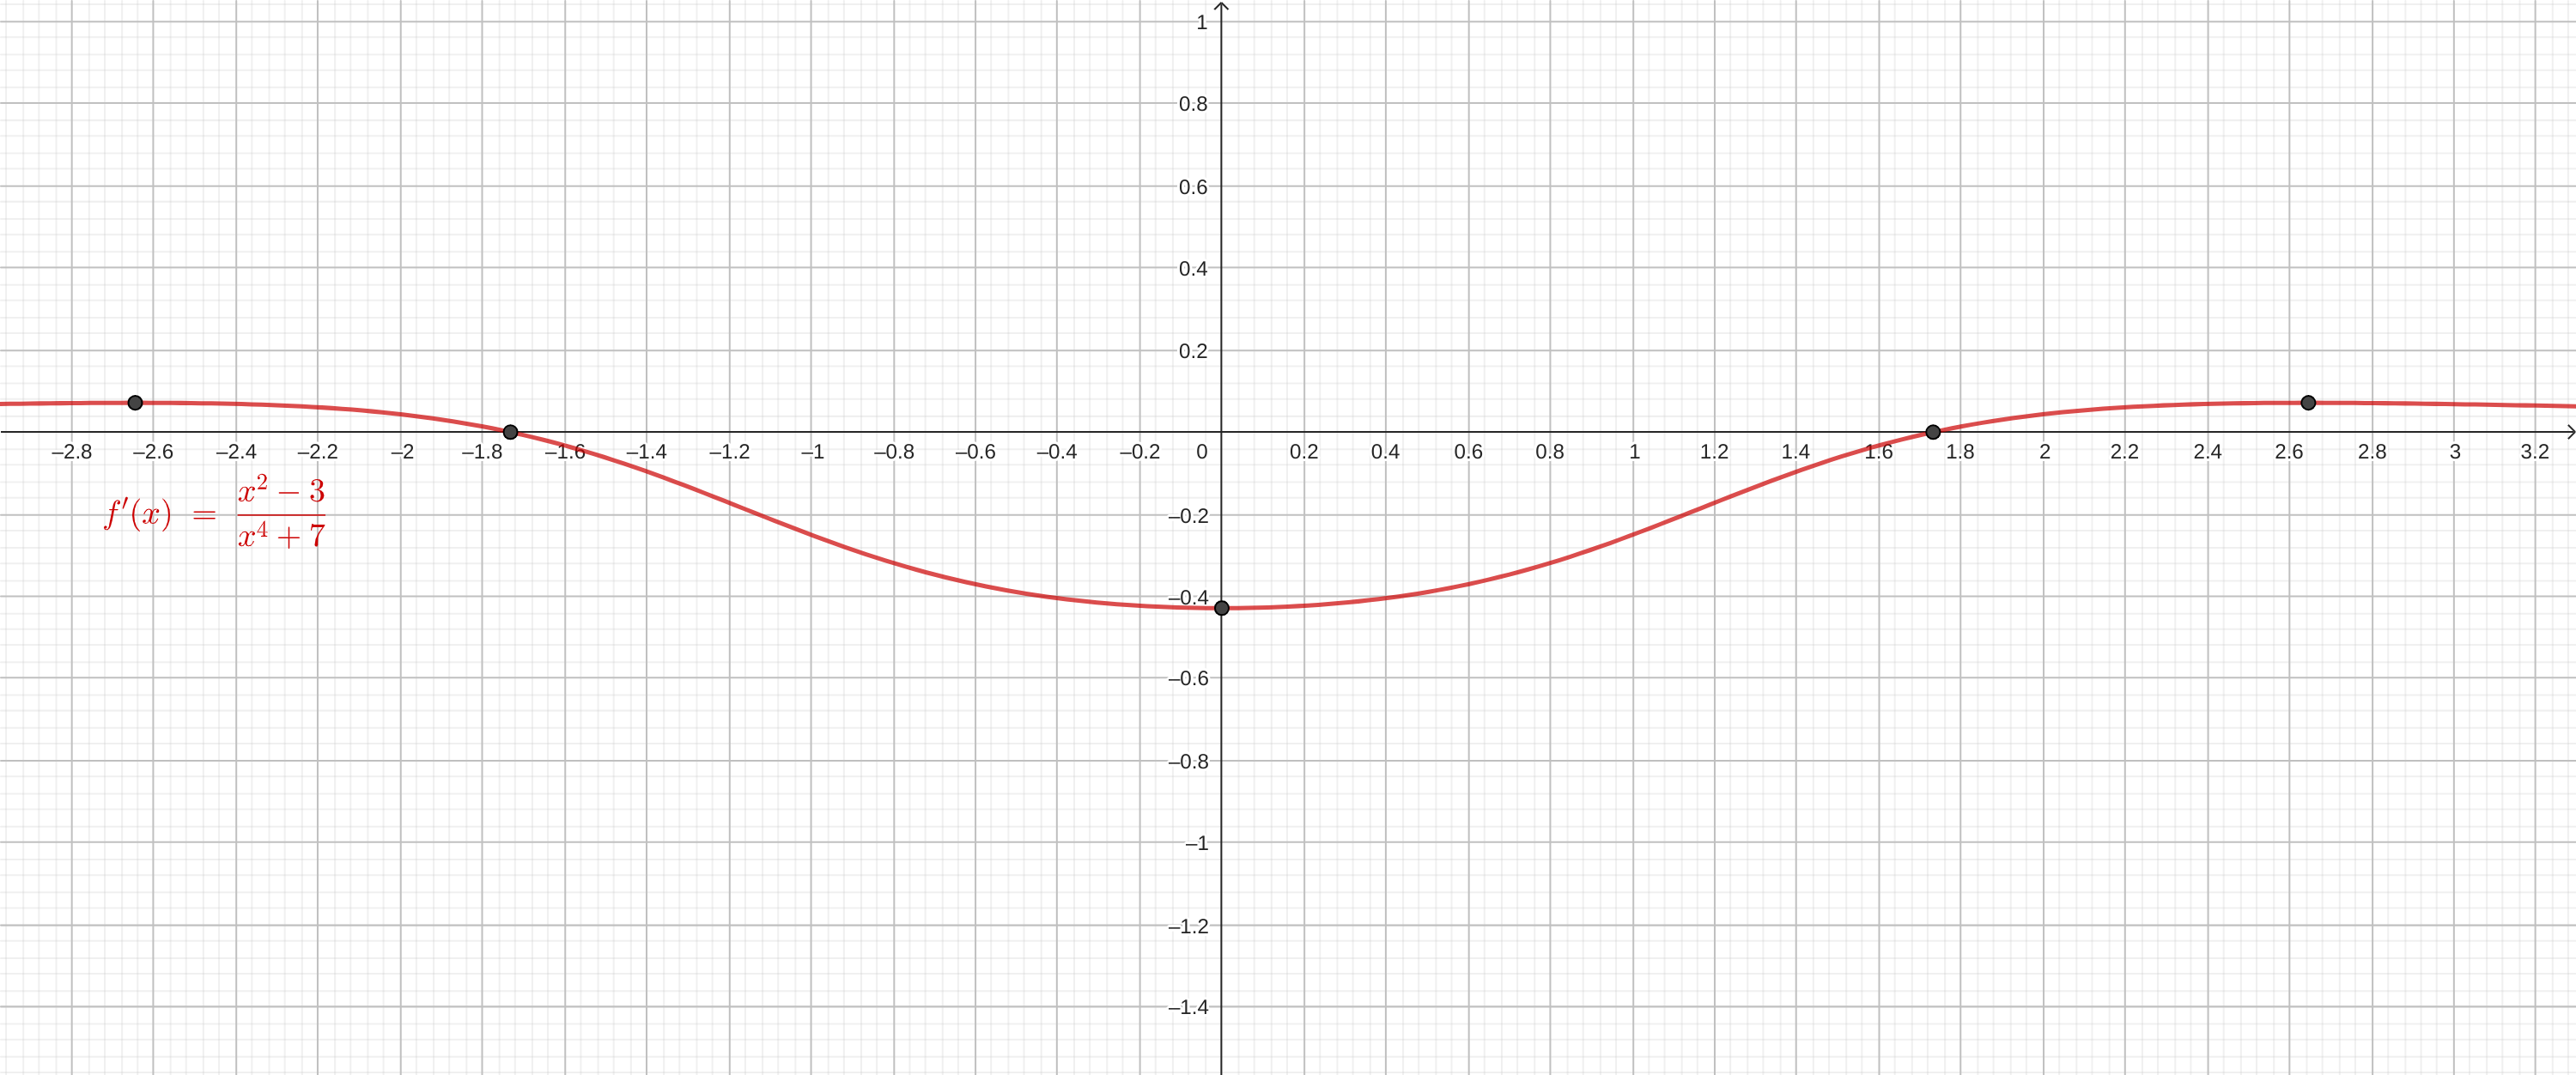
\includegraphics[height=7cm]{./imagenes/ej56.png}

% ---- 06. Ejercicio 64 LUIS ---- %
\section{Ejercicio 64, cap V Review Exercises.}
\paragraph*{64. Encuentra el valor promedio de \( f(x) = e^x + e^{-x} \) en el intervalo \([ \ln\frac{1}{2}, \ln 2 ]\).}
El valor promedio de una función en un intervalo $[a,b]$ se calcula mediante:

$$\overline{f}=\frac{1}{b-a}\int_a^b f(x)dx$$

Donde:
\begin{align*}
a &= \ln \frac{1}{2} \\
b &= \ln 2 \\
f(x) &= e^x + e^{-x}
\end{align*}

Entonces:
$$\overline{f}=\frac{1}{\ln 2-\ln \frac{1}{2}}\int_{\ln \frac{1}{2}}^{\ln 2} (e^x+e^{-x})dx$$

Para la integral:
$$\int (e^x+e^{-x})dx = e^x-e^{-x}+C$$

Evaluando en los límites:
\begin{align*}
[e^x-e^{-x}]_{\ln \frac{1}{2}}^{\ln 2} &= (e^{\ln 2}-e^{-\ln 2})-(e^{\ln \frac{1}{2}}-e^{-\ln \frac{1}{2}}) \\
&= (2-\frac{1}{2})-(\frac{1}{2}-2) \\
&= (2-\frac{1}{2})+(2-\frac{1}{2}) \\
&= 2(2-\frac{1}{2}) \\
&= 2(\frac{3}{2}) \\
&= 3
\end{align*}

Para el denominador:
\begin{align*}
\ln 2-\ln \frac{1}{2} &= \ln 2-(-\ln 2) \\
&= 2\ln 2
\end{align*}

Por lo tanto:
$$\overline{f}=\frac{3}{2\ln 2}$$

% ---- 07. Ejercicio 68 IHEBEL ---- %
\section{Ejercicio 68, cap V Review Exercises.}
Encuentra la función de posición de la particula que se mueve en el eje \textit{s}
\begin{equation*}
  \begin{split}
    a(t)=4cos(2t)\\
    v(0)=-1\\
    s(0)=-3
  \end{split}
\end{equation*}
Recordamos que la aceleracion es la derivada de la velocidad y la velocidad es la derivada de la posición.\\
Entonces...
\begin{equation*}
  v(t)=\int 4\cos(2t)dt = 4 \int \cos(2t)dt
\end{equation*}
considerando
\begin{equation*}
  \begin{split}
    u &= 2t\\
    du &= 2dt\\
    \frac{du}{2} &= dt
  \end{split}
\end{equation*}
Sustituyendo
\begin{equation*}
  \begin{split}
    4 \int \frac{\cos(u)du}{2} &= 2\int\cos(u)du\\
    &= 2\sin(u)\\
    &= 2\sin(2t)+c
  \end{split}
\end{equation*}
Esto es una familia de funciones, pero sabemos que $v(0)=-1$, entonces igualamos
\begin{equation*}
  \begin{split}
    2\sin(2(0))+c &= -1\\
    2\sin(0)+c &= -1\\
    c &= -1
  \end{split}
\end{equation*}
Por lo tanto
\begin{equation*}
  v(t)=2\sin(2t)-1
\end{equation*}
Ahora para obtener la funcion $s(t)$
\begin{equation*}
  \begin{split}
    s(t)&=\int (2\sin(2t)-1) dt\\
    &= \int 2\sin(2t)dt - \int dt\\
    &= 2\int\sin(2t)dt - t
  \end{split}
\end{equation*}
Consideramos
\begin{equation*}
  \begin{split}
    u &= 2t\\
    du &= 2dt\\
    \frac{du}{2} &= dt
  \end{split}
\end{equation*}
Sustituyendo
\begin{equation*}
  \begin{split}
    2\int \frac{\sin(u)du}{2}-t &= \int \sin(u)du + t\\
    &= -\cos(u)-t\\
    &= -\cos(2t)-t+c
  \end{split}
\end{equation*}
Caso similar al anterior, tenemos ahora una familia de funciones, pero sabemos que $s(0)=-3$, por lo tanto
\begin{equation*}
  \begin{split}
    -\cos(2(0))-(0)+c &= -3\\
    -\cos(0)+c &= -3\\
    -1+c &= -3 \\
    c &= -3 + 1\\
    c &= -2
  \end{split}
\end{equation*}
Por lo tanto, la ecuación de posición $s(t)$ está dada por
\begin{equation*}
  s(t)=-\cos(2t)-t-2
\end{equation*}

% ---- 08. Ejercicio 73 LUIS ---- %
\section{Ejercicio 73, cap V Review Exercises.}
\paragraph*{Una partícula se mueve con una velocidad de v(t) m/s a lo largo de un eje s. Encuentra el desplazamiento y la distancia recorrida por la partícula durante el intervalo de tiempo dado.}

\begin{equation*}
    v(t) = \frac{1}{2} - \frac{1}{t^2}; \quad 1 \leq t \leq 3
\end{equation*}

Dada la velocidad $v(t) = \frac{1}{2} - \frac{1}{t^2}$ para $1 \leq t \leq 3$

\subsection*{Desplazamiento}

El desplazamiento se calcula integrando la velocidad:

\begin{align*}
\text{Desplazamiento} &= \int_{1}^{3} \left(\frac{1}{2} - \frac{1}{t^2}\right)dt \\
&= \int_{1}^{3} \frac{1}{2}dt - \int_{1}^{3} \frac{1}{t^2}dt \\
&= \left[\frac{1}{2}t + \frac{1}{t}\right]_{1}^{3} \\
&= \left(\frac{1}{2}(3) + \frac{1}{3}\right) - \left(\frac{1}{2}(1) + 1\right) \\
&= \left(1.5 + \frac{1}{3}\right) - (0.5 + 1) \\
&= 1.83 - 1.5 \\
&= 0.33 \text{ metros}
\end{align*}

\subsection*{Distancia Recorrida}

Para la distancia recorrida, necesitamos $|v(t)| = \left|\frac{1}{2} - \frac{1}{t^2}\right|$

Encontramos el punto donde $v(t) = 0$:
\begin{align*}
\frac{1}{2} - \frac{1}{t^2} &= 0 \\
\frac{1}{2} &= \frac{1}{t^2} \\
t^2 &= 2 \\
t &= \sqrt{2} = 1.414
\end{align*}

Como $\sqrt{2}$ está en $[1,3]$, la partícula cambia de dirección.


\begin{align*}
  \text{Distancia} &= \int_{1}^{\sqrt{2}} \left|-\left(\frac{1}{2} - \frac{1}{t^2}\right)\right|dt + \int_{\sqrt{2}}^{3} \left|\frac{1}{2} - \frac{1}{t^2}\right|dt \\
  &= \int_{1}^{\sqrt{2}} \left(\frac{1}{t^2} - \frac{1}{2}\right)dt + \int_{\sqrt{2}}^{3} \left(\frac{1}{2} - \frac{1}{t^2}\right)dt \\
  &= \left[-\frac{1}{t} - \frac{1}{2}t\right]_{1}^{\sqrt{2}} + \left[\frac{1}{2}t + \frac{1}{t}\right]_{\sqrt{2}}^{3} \\
  &= \left(-\frac{1}{\sqrt{2}} - \frac{\sqrt{2}}{2}\right) - \left(-1 - \frac{1}{2}\right) + \left(\frac{3}{2} + \frac{1}{3}\right) - \left(\frac{\sqrt{2}}{2} + \frac{1}{\sqrt{2}}\right) \\
  &= \left(-\frac{1}{\sqrt{2}} - \frac{\sqrt{2}}{2} + 1.5\right) + \left(\frac{3}{2} + \frac{1}{3} - \frac{\sqrt{2}}{2} - \frac{1}{\sqrt{2}}\right) \\
  & = 0.7120 \text{ metros}
  \end{align*}

% ---- 09. Ejercicio 76 YAMILE ---- %
\section{Ejercicio 76, cap V Review Exercises.}
\section*{Cálculo del desplazamiento y la distancia total recorrida}

Dada la aceleración \(a(t) = \frac{1}{\sqrt{5t + 1}}\) m/s\(^2\) y la velocidad inicial \(v_0 = 2\) m/s, queremos calcular el desplazamiento y la distancia total recorrida por la partícula en el intervalo \(0 \leq t \leq 3\).

\subsection*{Paso 1: Encontrar la velocidad \(v(t)\)}

Sabemos que:
\[
a(t) = \frac{dv}{dt}.
\]

Por lo tanto, la velocidad se obtiene integrando \(a(t)\):
\[
v(t) = \int a(t) \, dt = \int \frac{1}{\sqrt{5t + 1}} \, dt.
\]

Para resolver la integral, usamos el cambio de variable:
\[
u = 5t + 1 \quad \Rightarrow \quad du = 5 \, dt \quad \Rightarrow \quad dt = \frac{du}{5}.
\]

La integral se convierte en:
\[
\int \frac{1}{\sqrt{5t + 1}} \, dt = \int \frac{1}{\sqrt{u}} \cdot \frac{1}{5} \, du = \frac{1}{5} \int u^{-1/2} \, du = \frac{1}{5} \cdot 2u^{1/2} + C.
\]

Sustituyendo \(u = 5t + 1\), obtenemos:
\[
v(t) = \frac{2}{5} \sqrt{5t + 1} + C.
\]

Usamos la condición inicial \(v(0) = 2\) para calcular \(C\):
\[
v(0) = \frac{2}{5} \sqrt{5(0) + 1} + C = 2 \quad \Rightarrow \quad \frac{2}{5}(1) + C = 2 \quad \Rightarrow \quad C = \frac{8}{5}.
\]

Por lo tanto, la expresión para la velocidad es:
\[
v(t) = \frac{2}{5} \sqrt{5t + 1} + \frac{8}{5}.
\]

\subsection*{Paso 2: Calcular el desplazamiento}

El desplazamiento se obtiene integrando \(v(t)\) en el intervalo \(0 \leq t \leq 3\):
\[
\text{Desplazamiento} = \int_{0}^{3} v(t) \, dt = \int_{0}^{3} \left( \frac{2}{5} \sqrt{5t + 1} + \frac{8}{5} \right) \, dt.
\]

Separamos en dos integrales:
\[
\int_{0}^{3} v(t) \, dt = \frac{2}{5} \int_{0}^{3} \sqrt{5t + 1} \, dt + \frac{8}{5} \int_{0}^{3} 1 \, dt.
\]

\subsubsection*{Primera integral}
Usamos nuevamente el cambio de variable \(u = 5t + 1\), con \(du = 5 \, dt\) y \(dt = \frac{du}{5}\). Los límites de integración cambian:
\[
t = 0 \Rightarrow u = 1, \quad t = 3 \Rightarrow u = 16.
\]

La integral se convierte en:
\[
\int_{0}^{3} \sqrt{5t + 1} \, dt = \int_{1}^{16} \sqrt{u} \cdot \frac{1}{5} \, du = \frac{1}{5} \int_{1}^{16} u^{1/2} \, du = \frac{1}{5} \cdot \frac{2}{3} \left[ u^{3/2} \right]_{1}^{16}.
\]

Evaluamos:
\[
\int_{0}^{3} \sqrt{5t + 1} \, dt = \frac{2}{15} \left[ (16)^{3/2} - (1)^{3/2} \right] = \frac{2}{15} \left[ 64 - 1 \right] = \frac{2}{15} \cdot 63 = \frac{126}{15} = 8.4.
\]

Por lo tanto:
\[
\frac{2}{5} \int_{0}^{3} \sqrt{5t + 1} \, dt = \frac{2}{5} \cdot 8.4 = 3.36.
\]

\subsubsection*{Segunda integral}
La segunda integral es:
\[
\int_{0}^{3} 1 \, dt = [t]_{0}^{3} = 3.
\]

Por lo tanto:
\[
\frac{8}{5} \int_{0}^{3} 1 \, dt = \frac{8}{5} \cdot 3 = 4.8.
\]

\subsubsection*{Resultado del desplazamiento}
Sumamos ambas partes:
\[
\text{Desplazamiento} = 3.36 + 4.8 = 8.16 \, \text{m}.
\]

\subsection*{Paso 3: Calcular la distancia total recorrida}

La velocidad \(v(t)\) es positiva en todo el intervalo \(0 \leq t \leq 3\), ya que \(\frac{2}{5} \sqrt{5t + 1} > 0\) y \(\frac{8}{5} > 0\). Por lo tanto, la distancia total recorrida es igual al desplazamiento.

\subsection*{Resultado final}
\begin{itemize}
    \item \textbf{Desplazamiento}: \(8.16 \, \text{m}\).
    \item \textbf{Distancia total recorrida}: \(8.16 \, \text{m}\).
\end{itemize}

% ---- 10. Ejercicio 85 IHEBEL ---- %
\section{Ejercicio 85, cap V Review Exercises.}
Evaluar la integral por sustitución,
\begin{equation*}
  \int_0^1\sin^2(\pi x)\cos(\pi x)dx
\end{equation*}
Considerando:
\begin{equation*}
  \begin{split}
    u &= \sin(\pi x)\\
    du &= \cos(\pi x)\pi dx\\
    u^2 &= \sin^2(\pi x)\\
    u(0)&=\sin(\pi (0))=\sin(0)=0\\
    u(1) &= \sin(\pi (1)) = \sin(\pi))=0
  \end{split}
\end{equation*}
Sustituimos.
\begin{equation*}
  \pi \int_0^0u^2 \frac{\cos(\pi x)du}{\cos(2\pi)} = \pi \int_0^0 u^2du
\end{equation*}
Como el límite de integración superior es igual al inferior, el área bajo la curva dada es de 0.
\begin{equation*}
  \pi \int_0^0 u^2du = \pi (0) = 0
\end{equation*}
Por lo tanto, el valor de la integral es 0

%\section*{2da Parte}

\subparagraph{Ejercicios: Review Exercises Capítulo 6 Anton-Bivens-Davis (pp. 485-486).}

% ---- 11. Ejercicio 7 YAMILE ---- %
\section{Ejercicio 7, cap VI Review Exercises.}
\section*{Problema: Área encerrada entre \( y = x^3 \) y \( y = x \) en \([-1, 2]\)}

Queremos calcular el área total encerrada entre las curvas \( y = x^3 \) y \( y = x \) en el intervalo \([-1, 2]\). 

\subsection*{Paso 1: Encontrar los puntos de intersección}
Para encontrar los puntos de intersección, resolvemos:
\[
x^3 = x \quad \Rightarrow \quad x(x^2 - 1) = 0 \quad \Rightarrow \quad x = 0, \, x = -1, \, x = 1.
\]

Por lo tanto, las curvas se intersectan en \( x = -1 \), \( x = 0 \) y \( x = 1 \).

\subsection*{Paso 2: Determinar cuál curva es mayor en cada intervalo}
\begin{itemize}
 \item En \([-1, 0]\), la curva \( y = x^3 \) está por debajo de \( y = x \).
 \item En \([0, 1]\), la curva \( y = x^3 \) también está por debajo de \( y = x \).
 \item En \([1, 2]\), la curva \( y = x^3 \) está por encima de \( y = x \).
\end{itemize}

\subsection*{Paso 3: Configuración de las integrales}
El área total se calcula como:
\[
A_{\text{total}} = \int_{-1}^0 \big(x - x^3\big) \, dx + \int_0^1 \big(x - x^3\big) \, dx + \int_1^2 \big(x^3 - x\big) \, dx.
\]

\subsection*{Paso 4: Cálculo de las integrales}

\subsubsection*{Primera integral: \( \int_{-1}^0 \big(x - x^3\big) \, dx \)}
\[
\int_{-1}^0 \big(x - x^3\big) \, dx = \int_{-1}^0 x \, dx - \int_{-1}^0 x^3 \, dx.
\]
Resolviendo término a término:
\[
\int_{-1}^0 x \, dx = \left[\frac{x^2}{2}\right]_{-1}^0 = \frac{0^2}{2} - \frac{(-1)^2}{2} = -\frac{1}{2},
\]
\[
\int_{-1}^0 x^3 \, dx = \left[\frac{x^4}{4}\right]_{-1}^0 = \frac{0^4}{4} - \frac{(-1)^4}{4} = -\frac{1}{4}.
\]
Entonces:
\[
\int_{-1}^0 \big(x - x^3\big) \, dx = -\frac{1}{2} - \left(-\frac{1}{4}\right) = -\frac{1}{4}.
\]

\subsubsection*{Segunda integral: \( \int_0^1 \big(x - x^3\big) \, dx \)}
\[
\int_0^1 \big(x - x^3\big) \, dx = \int_0^1 x \, dx - \int_0^1 x^3 \, dx.
\]
Resolviendo término a término:
\[
\int_0^1 x \, dx = \left[\frac{x^2}{2}\right]_0^1 = \frac{1^2}{2} - \frac{0^2}{2} = \frac{1}{2},
\]
\[
\int_0^1 x^3 \, dx = \left[\frac{x^4}{4}\right]_0^1 = \frac{1^4}{4} - \frac{0^4}{4} = \frac{1}{4}.
\]
Entonces:
\[
\int_0^1 \big(x - x^3\big) \, dx = \frac{1}{2} - \frac{1}{4} = \frac{1}{4}.
\]

\subsubsection*{Tercera integral: \( \int_1^2 \big(x^3 - x\big) \, dx \)}
\[
\int_1^2 \big(x^3 - x\big) \, dx = \int_1^2 x^3 \, dx - \int_1^2 x \, dx.
\]
Resolviendo término a término:
\[
\int_1^2 x^3 \, dx = \left[\frac{x^4}{4}\right]_1^2 = \frac{2^4}{4} - \frac{1^4}{4} = \frac{16}{4} - \frac{1}{4} = \frac{15}{4},
\]
\[
\int_1^2 x \, dx = \left[\frac{x^2}{2}\right]_1^2 = \frac{2^2}{2} - \frac{1^2}{2} = \frac{4}{2} - \frac{1}{2} = \frac{3}{2}.
\]
Entonces:
\[
\int_1^2 \big(x^3 - x\big) \, dx = \frac{15}{4} - \frac{3}{2} = \frac{15}{4} - \frac{6}{4} = \frac{9}{4}.
\]

\subsection*{Paso 5: Área total}
Sumando las tres integrales:
\[
A_{\text{total}} = \left(-\frac{1}{4}\right) + \frac{1}{4} + \frac{9}{4} = \frac{9}{4}.
\]

\subsection*{Resultado final}
El área encerrada entre las curvas es:
\[
\boxed{A_{\text{total}} = \frac{9}{4}}
\]

% ---- 12. Ejercicio 13 LUIS ---- %
\section{Ejercicio 13, cap VI Review Exercises.}
\paragraph*{Encuentra la longitud de arco en el segundo cuadrante de la curva:}
\begin{equation*}
    x^{2/3} + y^{2/3} = 4, \quad \text{desde } x = -8 \text{ hasta } x = -1
\end{equation*}

\subsection*{Fórmula para la Longitud de Arco}
La longitud de arco $L$ de una curva definida por $y = f(x)$ entre $x = a$ y $x = b$ usaremos la f\'ormula:

\begin{equation*}
  L = \int_{a}^{b} \sqrt{1 + \left(\frac{dy}{dx}\right)^2} dx
\end{equation*}

Iniciaremos despejando a $y$:

\begin{equation*}
  y^{2/3} = 4 - x^{2/3}
\end{equation*}

\begin{equation*}
  y = \left( 4 - x^{2/3} \right)^{3/2}
\end{equation*}
Como estamos en el segundo cuadrante, debemos tener $x < 0$, y el valor de $y$ debe ser positivo.

\subsection*{Derivamos la Función $y(x)$}
Primero derivamos $y$ respecto a $x$:

\begin{equation*}
  y = \left( 4 - x^{2/3} \right)^{3/2}
\end{equation*}

Usando la regla de la cadena:

\begin{equation*}
  \frac{dy}{dx} = \frac{3}{2} \left( 4 - x^{2/3} \right)^{1/2} \cdot \left( -\frac{2}{3} x^{-1/3} \right)
\end{equation*}

\begin{equation*}
  \frac{dy}{dx} = -\frac{1}{x^{1/3}} \left( 4 - x^{2/3} \right)^{1/2}
\end{equation*}

\subsection*{Sustituir en la Fórmula de la Longitud de Arco}
Ahora sustituimos $\frac{dy}{dx}$ en la f\'ormula de la longitud de arco:

\begin{equation*}
  L = \int_{-8}^{-1} \sqrt{1 + \left( -\frac{1}{x^{1/3}} \left( 4 - x^{2/3} \right)^{1/2} \right)^2} \, dx
\end{equation*}

\begin{equation*}
  L = \int_{-8}^{-1} \sqrt{1 + \frac{(4 - x^{2/3})}{x^{2/3}}} \, dx
\end{equation*}

Finalmente calculamos la integral:
\begin{align*}
    L &= \int_{-8}^{-1} \sqrt{1 + \frac{4-x^{2/3}}{x^{2/3}}} \, dx \\
    &= \int_{-8}^{-1} \sqrt{\frac{x^{2/3} + 4-x^{2/3}}{x^{2/3}}} \, dx \\
    &= \int_{-8}^{-1} \sqrt{\frac{4}{x^{2/3}}} \, dx = 9
    \end{align*}


% ---- 13. Ejercicio 16 YAMILE ---- %
\section{Ejercicio 16, cap VI Review Exercises.}
\section*{Problema de Superficies de Revolución}

Sea la curva \( 27x - y^3 = 0 \) en el intervalo \( y = 0 \) a \( y = 2 \). Vamos a encontrar las integrales necesarias para resolver las áreas de las superficies generadas por la rotación de esta curva alrededor de distintos ejes.

\subsection*{Información preliminar}

La curva está dada por:
\[
27x - y^3 = 0 \quad \Rightarrow \quad x = \frac{y^3}{27}.
\]
La derivada de \(x\) con respecto a \(y\) es:
\[
\frac{dx}{dy} = \frac{d}{dy}\left(\frac{y^3}{27}\right) = \frac{3y^2}{27} = \frac{y^2}{9}.
\]
El diferencial de arco en términos de \(y\) es:
\[
ds = \sqrt{1 + \left(\frac{dx}{dy}\right)^2} \, dy = \sqrt{1 + \left(\frac{y^2}{9}\right)^2} \, dy = \sqrt{1 + \frac{y^4}{81}} \, dy.
\]

\subsection*{(a) Revolver alrededor del eje \(x\) (respecto a \(x\))}

Para calcular el área de la superficie de revolución alrededor del eje \(x\), necesitamos expresar \(y\) como función de \(x\). A partir de \( 27x = y^3 \), tenemos:
\[
y = (27x)^{1/3}.
\]
La derivada de \(y\) con respecto a \(x\) es:
\[
\frac{dy}{dx} = \frac{d}{dx} ((27x)^{1/3}) = \frac{1}{3} (27x)^{-2/3} \cdot 27 = 9x^{-2/3}.
\]
El diferencial de arco en términos de \(x\) es:
\[
ds = \sqrt{1 + \left(\frac{dy}{dx}\right)^2} \, dx = \sqrt{1 + (9x^{-2/3})^2} \, dx = \sqrt{1 + 81x^{-4/3}} \, dx.
\]
El área de la superficie generada al rotar alrededor del eje \(x\) es:
\[
A_x = 2\pi \int_{x_1}^{x_2} y \, ds,
\]
donde los límites de integración son los valores de \(x\) correspondientes a \(y = 0\) y \(y = 2\). Entonces, tenemos:
\[
x_1 = \frac{(0)^3}{27} = 0, \quad x_2 = \frac{(2)^3}{27} = \frac{8}{27}.
\]
Por lo tanto, el área es:
\[
A_x = 2\pi \int_{0}^{\frac{8}{27}} (27x)^{1/3} \sqrt{1 + 81x^{-4/3}} \, dx.
\]

\subsection*{(b) Revolver alrededor del eje \(y\) (respecto a \(y\))}

Para calcular el área de la superficie generada al rotar alrededor del eje \(y\), usamos:
\[
A_y = 2\pi \int_{y_1}^{y_2} x \, ds,
\]
donde los límites de integración son \(y_1 = 0\) y \(y_2 = 2\). Sustituyendo \(x = \frac{y^3}{27}\) y \(ds = \sqrt{1 + \frac{y^4}{81}} \, dy\), el área es:
\[
A_y = 2\pi \int_{0}^{2} \frac{y^3}{27} \sqrt{1 + \frac{y^4}{81}} \, dy.
\]


\subsection*{(c) Revolver alrededor de la línea \(y = -2\) (respecto a \(y\))}

Cuando rotamos alrededor de una línea distinta del eje, la distancia al eje de rotación cambia. En este caso, la distancia entre un punto en la curva y la línea \(y = -2\) es:
\[
\text{Distancia} = y - (-2) = y + 2.
\]
El área de la superficie generada es:
\[
A = 2\pi \int_{y_1}^{y_2} \text{(Distancia)} \cdot x \, ds.
\]
Sustituyendo \(\text{Distancia} = y + 2\), \(x = \frac{y^3}{27}\), y \(ds = \sqrt{1 + \frac{y^4}{81}} \, dy\), el área es:
\[
A = 2\pi \int_{0}^{2} (y + 2) \cdot \frac{y^3}{27} \sqrt{1 + \frac{y^4}{81}} \, dy.
\]

\subsection*{Resumen de las integrales}

1. **Revolución alrededor del eje \(x\):**
\[
A_x = 2\pi \int_{0}^{\frac{8}{27}} (27x)^{1/3} \sqrt{1 + 81x^{-4/3}} \, dx.
\]

2. **Revolución alrededor del eje \(y\):**
\[
A_y = 2\pi \int_{0}^{2} \frac{y^3}{27} \sqrt{1 + \frac{y^4}{81}} \, dy.
\]

3. **Revolución alrededor de \(y = -2\):**
\[
A = 2\pi \int_{0}^{2} (y + 2) \cdot \frac{y^3}{27} \sqrt{1 + \frac{y^4}{81}} \, dy.
\]


% ---- 14. Ejercicio 19 IHEBEL ---- %
\section{Ejercicio 19, cap VI Review Exercises.}
\textbf{a)} Un resorte ejerce una fuerza de 0.5N cuando es estirado más de su longitud natural.
Asumiendo que aplica la ley de Hooke, ¿cuánto trabajo fue efectuado al estar el resorte a esa longitud?\\
\textbf{b)} ¿Qué tanto trabajo más de su longitud natural se estiraría al aplicar 25J de trabajo?
\subsection*{a)}
Utilizaremos las formulas:\\
\begin{equation*}
  w=\int_{a}^{b}F(x)dx
\end{equation*}
\begin{equation*}
  \begin{split}
    F(x) &= kx\\
    \frac{F(x)}{x} &= k
  \end{split}
\end{equation*}
Primero calculamos la constante k
\begin{equation*}
  k=\frac{F(x)}{x}=\frac{0.5}{0.25}=2
\end{equation*}
de aquí $F(x)=2x$.\\
Ahora calculamos el trabajo.
\begin{equation*}
  \begin{split}
    w &= \int_{0}^{0.25}2xdx\\
    &= \left[ \frac{2}{2}x^2\right]^{0.25}_{0}\\
    &=(0.25)^2-(0)\\
    &=0.0625
  \end{split}
\end{equation*}
El trabajo realizado para estirar el resorte a 0.25m es 0.0675J.

\subsection*{b)}
Queremos calcular la distancia d, entonces, cambiamos la integral que sabemos que tiene un valor de 25J
\begin{equation*}
  \begin{split}
    \int_{0}^{d}2xdx &= 25\\
        [x^2]_{0}^{d} &=25\\
        (d)^2-(0)^2 &=25\\
        d^2 &=25\\
        d&=5
  \end{split}
\end{equation*}
Por lo tanto, la distancia es de 5 metros

\subparagraph{Ejercicios: Review Exercises Capítulo 7 Anton-Bivens-Davis (pp. 557-559).}

% ---- 15. Ejercicio 8 IHEBEL ---- %
\section{Ejercicio 8, cap VII Review Exercises.}
Evaluar la integral
\begin{equation*}
  \int_{0}^{1} \frac{x^3dx}{\sqrt{x^2+1}}
\end{equation*}
por:\\
\textit{a)} Integral por partes.\\
\textit{b)} Sustituyendo con $u=\sqrt{x^2+1}$.
\subsection*{a) Integral por partes}
Considerando
\begin{equation*}
  \begin{split}
    u &= x^2\\
    du &= 2xdx\\
    \\
    dv &= x(x^2+1)^{-{\frac{1}{2}}}\\
    v &= \int \frac{x}{\sqrt{x^2+1}}dx
  \end{split}
\end{equation*}
consideramos
\begin{equation*}
  \begin{split}
    a &= x^2+1\\
    da &= 2xdx\\
    \frac{da}{2x} &= dx
  \end{split}
\end{equation*}
\begin{equation*}
  \begin{split}
    v &= \int \frac{xda}{2x\sqrt{a}}\\
    &= \frac{1}{2} \int \frac{da}{\sqrt{a}}\\
    &= a^{\frac{1}{2}}\\
    &= \sqrt{x^2=1}
  \end{split}
\end{equation*}
Sustiuyendo usando la formula de integracion por partes
\begin{equation*}
  \int u dv = uv - \int v du
\end{equation*}
Tenemos
\begin{equation*}
    \int \frac{xx^2}{\sqrt{x^2+1}}dx=x^2\sqrt{x^2+1}-\int\sqrt{x^2+1}2xdx
\end{equation*}
Aplicamos sustitución considerando
\begin{equation*}
  \begin{split}
    a &= x^2+1\\
    da &= 2xdx\\
    \frac{da}{2x} &= dx
  \end{split}
\end{equation*}
\begin{equation*}
  \begin{split}
    \int\frac{\sqrt{a}2xda}{2x} &= \int \sqrt{a}da\\
    &=\frac{2}{3}a^{\frac{3}{2}}\\
    &=\frac{2}{3}(x^2+1)^{\frac{3}{2}}+c
  \end{split}
\end{equation*}
Ahora evaluamos en los limites dados
\begin{equation*}
  \begin{split}
    \int_{0}^{1}\frac{x^3}{\sqrt{x^2+1}} &= \left[ x^2\sqrt{x^2+1}-\frac{2}{3}(x^2+1)^{\frac{3}{2}}\right]^{1}_{0}\\
    &=\left((1)^2\sqrt{(1)^2+1}-\frac{2}{3}((1)^2+1)^{\frac{3}{2}}\right) - \left(\underbrace{(0)^2\sqrt{(0)^2+1}}_{0}-\frac{2}{3}\underbrace{((0)^2+1)^{\frac{3}{2}}}_{1}\right)\\
    &=2^{\frac{1}{2}}-\frac{2}{3}(2)^{\frac{3}{2}}+\frac{2}{3}\\
    &=2^{\frac{1}{2}}(1-\frac{2}{3}(2))+\frac{2}{3}\\
    &=2^{\frac{1}{2}}(\frac{3}{3}-\frac{4}{3})+\frac{2}{3}\\
    &=2^{\frac{1}{2}}(-\frac{1}{3})+\frac{2}{3}\\
    &=\frac{2}{3}-\frac{\sqrt{2}}{3}\\
    &=\frac{2-\sqrt{2}}{3}
  \end{split}
\end{equation*}

\subsection*{b) Sustitucion}
Consideramos
\begin{equation*}
  \begin{split}
    u &= \sqrt{x^2+1} =(x^2+1)^{\frac{1}{2}}\\
    du &= \frac{1}{2}(x^2+1)^{-\frac{1}{2}}2xdx\\
    \frac{\sqrt{x^2+1}du}{x} &= dx\\
    u^2 &= x^2+1\\
    u^2-1 &= x^2\\
    \\
    u(1) &= \sqrt{(1)^2+1} = \sqrt{2} = (2)^{\frac{1}{2}}\\
    u(0) &= \sqrt{(0)^2+1} = 1
  \end{split}
\end{equation*}
Sustituimos
\begin{equation*}
  \begin{split}
    \int_{0}^{1} \frac{x^3}{\sqrt{x^2+1}}dx &= \int_{1}^{\sqrt{2}} \frac{x(u^2-1)\sqrt{x^2+1}du}{x\sqrt{x^2+1}}\\
    &= \int_{1}^{\sqrt{2}}(u^2-1)du\\
    &= \left( \frac{1}{3}(2^{\frac{1}{2}})^3-2^{\frac{1}{2}} \right) - \left( \frac{1}{3}(1)^{\frac{1}{2}}-1 \right)\\
    &=2^{\frac{1}{2}}\left( \frac{2}{3}-\frac{3}{3} \right)+\frac{2}{3}\\
    &=2^{\frac{1}{2}}\left( -\frac{1}{3}\right) + \frac{2}{3}\\
    &=-\frac{\sqrt{2}}{3}+\frac{2}{3}\\
    &=\frac{2-\sqrt{2}}{3}
  \end{split}
\end{equation*}
En ambos casos obtenemos el mismo resultado.

% ---- 16. Ejercicio 14 LUIS ---- %
\section{Ejercicio 14, cap VII Review Exercises.}
Una partícula moviéndose a lo largo del eje $x$ tiene una función de velocidad $v(t)=t^2e^{-t}$. ¿Qué distancia recorre la partícula desde $t=0$ hasta $t=5$?
\\
\\La distancia recorrida por la partícula está dada por:
\[
d = \int_0^5 |v(t)| \, dt
\]

\subsection*{Resolución de la integral}
Para resolver \( \int t^2 e^{-t} \, dt \), utilizamos el método de integración por partes:
\[
u = t^2, \quad dv = e^{-t} \, dt
\]
Entonces:
\[
du = 2t \, dt, \quad v = -e^{-t}
\]
Aplicando la fórmula de integración por partes:
\[
\int t^2 e^{-t} \, dt = -t^2 e^{-t} + \int 2t e^{-t} \, dt
\]

Ahora, resolvemos la integral \( \int 2t e^{-t} \, dt \) nuevamente por partes:
\[
u = 2t, \quad dv = e^{-t} \, dt \quad \Rightarrow \quad du = 2 \, dt, \quad v = -e^{-t}
\]
Entonces:
\[
\int 2t e^{-t} \, dt = -2t e^{-t} + \int 2e^{-t} \, dt
\]
La última integral es:
\[
\int 2e^{-t} \, dt = -2e^{-t}
\]
Por lo tanto:
\[
\int 2t e^{-t} \, dt = -2t e^{-t} - 2e^{-t}
\]

Sustituyendo este resultado en la expresión original:
\[
\int t^2 e^{-t} \, dt = -t^2 e^{-t} - 2t e^{-t} - 2e^{-t}
\]

\subsection*{Evaluamos los límites}
Evaluamos la integral en los límites \( t = 0 \) y \( t = 5 \):
\[
d = \left[ -t^2 e^{-t} - 2t e^{-t} - 2e^{-t} \right]_0^5
\]

Primero, evaluamos en \( t = 5 \):
\[
-t^2 e^{-t} - 2t e^{-t} - 2e^{-t} = -5^2 e^{-5} - 2(5)e^{-5} - 2e^{-5}
\]
\[
= -25e^{-5} - 10e^{-5} - 2e^{-5} = -37e^{-5}
\]

Luego, evaluamos en \( t = 0 \):
\[
-0^2 e^{0} - 2(0)e^{0} - 2e^{0} = -2
\]

Por lo tanto:
\[
d = \left(-37e^{-5} - (-2)\right) = 2 - 37e^{-5}
\]
\\El resultado será: 
\begin{equation*}
  d = 1.750
\end{equation*}


% ---- 17. Ejercicio 33 LUIS ---- %
\section{Ejercicio 33, cap VII Review Exercises.}
Considera la integral $\displaystyle\int \frac{1}{x^3 - x} dx$.

\begin{enumerate}[label=(\alph*)]
    \item Evalúa la integral usando la sustitución $x = \sec \theta$. 
    ¿Para qué valores de $x$ es válido tu resultado?

    \item Evalúa la integral usando la sustitución $x = \sin \theta$. 
    ¿Para qué valores de $x$ es válido tu resultado?

    \item Evalúa la integral usando el método de fracciones parciales. 
    ¿Para qué valores de $x$ es válido tu resultado?
\end{enumerate}

\subsection*{Inciso (a): Sustitución trigonométrica: $x = \sec \theta$}


Realizamos las sustituciones:
\begin{align*}
x &= \sec \theta \\
dx &= \sec \theta \tan \theta \, d\theta \\
x^3 - x &= \sec^3\theta - \sec \theta
\end{align*}

La integral se transforma en:
\begin{align*}
&\int \frac{1}{\sec^3\theta - \sec \theta} \sec \theta \tan \theta \, d\theta \\
&= \int \frac{\sec \theta \tan \theta}{\sec^3\theta - \sec \theta} \, d\theta \\
&= \int \frac{\tan \theta}{\sec^2\theta - 1} \, d\theta \\
&= \int \frac{\tan \theta}{\tan^2\theta} \, d\theta \\
&= \int \frac{1}{\tan \theta} \, d\theta \\
&= \ln|\sin \theta| + C
\end{align*}

Regresando a la variable original:
\[ \ln\left|\sqrt{1 - \frac{1}{x^2}}\right| + C \]

\textbf{Validez:} $|x| > 1$.

\subsection*{Inciso (b): Usando $x = \sin \theta$}

\begin{align*}
& \text{Sea } x = \sin \theta \\
& dx = \cos \theta \, d\theta \\
& x^3 - x = \sin^3\theta - \sin \theta = \sin \theta(\sin^2\theta - 1) = -\sin \theta \cos^2\theta \\
& \text{La integral se convierte en: } \int\frac{\cos \theta \, d\theta}{-\sin \theta \cos^2\theta} = -\int\frac{d\theta}{\sin \theta} \\
& \text{Esto nos da } -\ln|\cos \theta| \\
& \text{Como } x = \sin \theta, \text{ entonces } \cos \theta = \sqrt{1-x^2} \\
& \therefore \int\frac{1}{x^3-x}dx = \ln\left|\frac{\sqrt{1-x^2}}{x}\right| + C 
\end{align*}
\textbf{ Validez:} Es valido para $|x| < 1$

\subsection*{Inciso (c): M\'etodo de Fracciones Parciales}
Factorizamos el denominador:

\begin{equation*}
    \frac{1}{x(x-1)(x+1)} = \frac{A}{x} + \frac{B}{x-1} + \frac{C}{x+1}
\end{equation*}

Multiplicamos ambos lados por el denominador com\'un $x(x-1)(x+1)$:

\begin{equation*}
    1 = A(x-1)(x+1) + Bx(x+1) + Cx(x-1)
\end{equation*}

Expandiendo y agrupando t\'erminos similares:

\begin{equation*}
    1 = (A + B + C)x^2 + (B - C)x + (-A)
\end{equation*}

Para que esta igualdad sea cierta para todos los valores de $x$, los coeficientes deben ser iguales:

\begin{align*}
    A + B + C &= 0 \\
    B - C &= 0 \\
    -A &= 1
\end{align*}

De la tercera ecuaci\'on, obtenemos $A = -1$. De la segunda ecuaci\'on, $B = C$. De la primera ecuaci\'on:

\begin{equation*}
    -1 + B + B = 0 \implies B = \frac{1}{2}, \quad C = \frac{1}{2}
\end{equation*}

Por lo tanto:

\begin{equation*}
    \frac{1}{x(x-1)(x+1)} = \frac{-1}{x} + \frac{1/2}{x-1} + \frac{1/2}{x+1}
\end{equation*}

Integrando ambos lados:

\begin{equation*}
    \int \, \frac{1}{x(x-1)(x+1)} \, dx = \int \left( \frac{-1}{x} + \frac{1/2}{x-1} + \frac{1/2}{x+1} \right) \, dx
\end{equation*}

\begin{equation*}
    = -\ln |x| + \frac{1}{2} \ln |x-1| + \frac{1}{2} \ln |x+1| + C
\end{equation*}

\begin{equation*}
    = \ln \left| \frac{\sqrt{(x-1)(x+1)}}{x} \right| + C
\end{equation*}

\textbf{Validez}: Este resultado es v\'alido siempre que $x \neq 0, \pm 1$.


% ---- 18. Ejercicio 41 IHEBEL ---- %
\section{Ejercicio 41, cap VII Review Exercises.}
Aproxima la integral
\begin{equation*}
  \int_1^3 \frac{1}{\sqrt{x+1}}dx
\end{equation*}
usando...\\
\textbf{a)} Aproximacion del punto medio $M_{10}$.\\
\textbf{b)} Aproximacion trapezoidal $T_{10}$.\\
\textbf{c)} Regla de Simpson para la aproximacion $S_{20}$.\\
En cada caso, encontrar el error absoluto.\\
Considerar al menos 5 décimas.
\subsection*{Valor real}
\begin{equation*}
  \begin{split}
    u &= x+1\\
    du &= dx\\
    u(1) &= (1)+1 = 2\\
    u(3) &= (3)+1 = 4 
  \end{split}
\end{equation*}
\begin{equation*}
  \begin{split}
    \int_1^3 \frac{1}{\sqrt{x+1}}dx &= \int_2^4 u^{-\frac{1}{2}}\\
    &=\left[ 2u^{\frac{1}{2}} \right]_2^4\\
    &=2\sqrt{4}-2\sqrt{2}\\
    &=2(2)-2\sqrt{2}\\
    &=4-2\sqrt{2}\\
    &\approx 1.17157 \ \text{con calculadora}
  \end{split}
  \end{equation*}
El valor real de la funcion $V_R$ es de 1.17157u.
  

\subsection*{a) Punto Medio $M_{10}$}
\begin{equation*}
  \int_a^b f(x)dx=\left( \frac{b-a}{n}\right)\left( y_{m_1}+y_{m_2}+...+y_{m_n}\right)
\end{equation*}
Tenemos que
\begin{equation*}
  \begin{split}
    \Delta x &= \left( \frac{b-a}{n} \right)\\
    x_i &= a+(i-(\frac{1}{2}))\Delta x
  \end{split}
\end{equation*}
Sustituyendo e interpretando la serie y.
\begin{equation*}
    \int_a^b f(x)dx = \frac{b-a}{n}\sum_{i=1}^n\left(f\left( a+(i-\frac{1}{2})(\frac{b-a}{n}) \right)\right)
\end{equation*}
Calculamos la diferencial de x
\begin{equation*}
  \Delta x = \frac{b-a}{n} = \frac{3-1}{10}+\frac{2}{10}=\frac{1}{5}
\end{equation*}
susituyendo, obtenemos la aproximación:
\begin{equation*}
  \begin{split}
    \int_1^3 \frac{1}{\sqrt{x+1}}dx &\approx \frac{1}{5}\sum_{i=1}^{10}\frac{1}{\sqrt{(1+(i-\frac{1}{2})(\frac{1}{5}))+1}}\\
    &\approx \frac{1}{5}\sum_{i=1}^{10}\frac{1}{\sqrt{\frac{1}{5}}(i-\frac{i}{2})}\\
    &\approx 1.17138 \ \ \text{Resolviendo con calculadora}
  \end{split}
\end{equation*}
El error es
\begin{equation*}
    E_A=\|V_R-T_{10} \|=1.9x10^{-4}
\end{equation*}
El valor de la aproximación es de 1.17138u con un error de $1.9x10^{-4}$


\subsection*{b) Trapezoidal $T_{10}$}
Tenemos primero que
\begin{equation*}
  \int_a^b f(x)dx=\left( \frac{b-a}{2n}\right)\left( y_0+2y_1+2y_2y+2+...+2y_{n-1}+y_n\right)
\end{equation*}
Luego, tenemos que
\begin{equation*}
  \begin{split}
    x_i &= a+i\Delta x\\
    y_i &= f(x_i)
  \end{split}
\end{equation*}
Entonces
\begin{equation*}
  \begin{split}
    \int_a^b f(x)dx &= \left( \frac{b-a}{2n}\right)\left( y_0+2y_1+2y_2y+2+...+2y_{n-1}+y_n\right)\\
    &=\left( \frac{\Delta x}{2}\right)\left( y_0+y_n+2y_1+2y_2y+2+...+2y_{n-1}\right)\\
    &=\left( \frac{\Delta x}{2}\right)\left( y_0+y_n+2\sum_{i=0}^{n-1}y_i \right)\\
    &=\left( \frac{\Delta x}{2}\right)\left( f(a)+f(b)+2\sum_{i=0}^{n-1}f(a+i\Delta x) \right)
  \end{split}
\end{equation*}
Sustituyendo para obtener la aproximación
\begin{equation*}
  \begin{split}
    \int_1^3 \frac{1}{\sqrt{x+1}}dx &\approx \frac{1}{10}\left( \frac{1}{\sqrt{2}}+\frac{1}{2}=2\sum_{i=1}^{9}\frac{1}{\sqrt{(1+\frac{x}{5})+1}} \right)\\
    &\approx 1.17195 \ \ \text{Evaluando con calculadora}
  \end{split}
\end{equation*}
El error es
\begin{equation*}
    E_A=\|V_R-T_{10} \|=3.8x10^{-4}.
\end{equation*}
El valor aproximado de la función es de 1.17195u con un error de $3.8x10^{-4}$

\subsection*{c) Regla de Simpson}
\begin{equation*}
  \begin{split}
    \int_a^b f(x)dx &= \frac{1}{3}\left( 2M_k+T_k \right)\\
    S_n = \frac{1}{3}\left( 2M_{\frac{n}{2}}+T_{\frac{n}{2}}  \right)
    \end{split}
\end{equation*}
Por lo tanto, la aproximación por regla de Simpson esta dada por
\begin{equation*}
  S_{20}\approx\frac{1}{3}\left( 2\underbrace{M_{10}}_{\text{a)}}+\underbrace{T_{10}}_{\text{b)}}\right)\approx 1.17187.
\end{equation*}

\begin{equation*}
    E_A=\|V_R-S_{20} \|=0
\end{equation*}
Con la regla de Simpson, la aproximacion es de 1.17187u, que es igual al valor real (considerando solo 5 décimas)

% ---- 19. Ejercicio 51 YAMILE ---- %
\section{Ejercicio 51, cap VII Review Exercises.}
\section*{Problema: Área bajo la curva}

Queremos encontrar el área encerrada entre el eje \(x\) y la curva 
\[
y = \frac{\ln x - 1}{x^2}, \quad \text{para } x \geq e.
\]

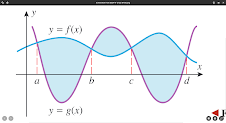
\includegraphics[height=7cm]{./imagenes/ej51.png}

\subsection*{Planteamiento del problema}

El área se calcula integrando la función \(y\) respecto a \(x\) desde \(x = e\) hasta el infinito. La integral a resolver es:
\[
A = \int_{e}^{\infty} \frac{\ln x - 1}{x^2} \, dx.
\]

---

\subsection*{Cálculo de la integral}

Descomponemos la integral en dos términos:
\[
A = \int_{e}^{\infty} \frac{\ln x}{x^2} \, dx - \int_{e}^{\infty} \frac{1}{x^2} \, dx.
\]

1. **Primer término: \(\int_{e}^{\infty} \frac{\ln x}{x^2} \, dx\)**

Sea \(u = \ln x\), por lo que \(du = \frac{1}{x} \, dx\). Sustituyendo \(x = e^u\), tenemos:
\[
\frac{\ln x}{x^2} \, dx = \frac{u}{e^{2u}} \, e^u \, du = u e^{-u} \, du.
\]

Por lo tanto, la integral se convierte en:
\[
\int_{e}^{\infty} \frac{\ln x}{x^2} \, dx = \int_{1}^{\infty} u e^{-u} \, du.
\]

Esta integral se resuelve por partes:
\[
\int u e^{-u} \, du = -u e^{-u} + \int e^{-u} \, du = -u e^{-u} - e^{-u} + C.
\]

Evaluando en los límites \(u = 1\) y \(u \to \infty\):
\[
\int_{1}^{\infty} u e^{-u} \, du = \left[ -u e^{-u} - e^{-u} \right]_{1}^{\infty}.
\]

Cuando \(u \to \infty\), \(u e^{-u} \to 0\) y \(e^{-u} \to 0\). Para \(u = 1\):
\[
\int_{1}^{\infty} u e^{-u} \, du = -1 e^{-1} - e^{-1} = -\frac{1}{e} - \frac{1}{e} = -\frac{2}{e}.
\]

Por lo tanto:
\[
\int_{e}^{\infty} \frac{\ln x}{x^2} \, dx = -\frac{2}{e}.
\]

2. **Segundo término: \(\int_{e}^{\infty} \frac{1}{x^2} \, dx\)**

La integral es:
\[
\int_{e}^{\infty} \frac{1}{x^2} \, dx = \left[ -\frac{1}{x} \right]_{e}^{\infty}.
\]

Cuando \(x \to \infty\), \(-\frac{1}{x} \to 0\). Para \(x = e\):
\[
\int_{e}^{\infty} \frac{1}{x^2} \, dx = -\frac{1}{\infty} - \left(-\frac{1}{e}\right) = \frac{1}{e}.
\]

---

\subsection*{Área total}

Sumando ambos términos:
\[
A = -\frac{2}{e} + \frac{1}{e} = -\frac{1}{e}.
\]

Como el área no puede ser negativa, tomamos el valor absoluto:
\[
A = \frac{1}{e}.
\]

---

\subsection*{Conclusión}

El área encerrada entre el eje \(x\) y la curva \(y = \frac{\ln x - 1}{x^2}\) para \(x \geq e\) es:
\[
A = \frac{1}{e}.
\]

% ---- 20. Ejercicio YAMILE ---- %
\section{Ejercicio: Classroom.}
\section*{Problema: Volumen del sólido restante al perforar una esfera}

Se perfora una esfera de radio \( R > 6 \, \mathrm{mm} \) mediante un túnel cilíndrico de 6 mm de largo que pasa por el centro de la esfera. Queremos demostrar que el volumen del sólido restante no depende del radio \( R \) y que es igual a \( 36\pi \, \mathrm{mm}^3 \). Usaremos el método de las cáscaras cilíndricas para calcular este volumen.

---

\subsection*{Configuración del problema}

1. **Ecuación de la esfera**: 
 La ecuación de una esfera centrada en el origen es:
 \[
 x^2 + y^2 + z^2 = R^2.
 \]

2. **Corte del túnel cilíndrico**: 
 El túnel cilíndrico es paralelo al eje \(z\) y tiene un radio de 6 mm. Esto significa que el cilindro está definido por:
 \[
 x^2 + y^2 \leq 6^2.
 \]

3. **Sólido restante**: 
 El volumen del sólido restante es el volumen de la esfera menos el volumen eliminado por el túnel y los casquetes esféricos.

---

\subsection*{Cálculo del volumen mediante cáscaras cilíndricas}

Para usar el método de las cáscaras cilíndricas, consideramos un cilindro elemental de radio \(x\), altura \(2z(x)\), y grosor diferencial \(dx\). La altura del cilindro viene dada por \(2z(x)\), donde \(z(x)\) es la coordenada \(z\) obtenida de la ecuación de la esfera:
\[
z(x) = \sqrt{R^2 - x^2}.
\]

La fórmula para el volumen elemental de una cáscara cilíndrica es:
\[
dV = \text{área lateral} \cdot dx = 2\pi x \cdot \text{altura} \cdot dx = 2\pi x \cdot 2z(x) \, dx.
\]

Sustituyendo \(z(x)\):
\[
dV = 2\pi x \cdot 2\sqrt{R^2 - x^2} \, dx = 4\pi x \sqrt{R^2 - x^2} \, dx.
\]

El volumen total se obtiene integrando \(dV\) sobre el intervalo donde \(x^2 + y^2 \leq 6^2\), es decir, para \(x \in [0, 6]\):
\[
V = \int_{0}^{6} 4\pi x \sqrt{R^2 - x^2} \, dx.
\]

---

\subsection*{Simplificación del cálculo}

Aunque \(R\) aparece en la integral, resulta que el volumen final no depende de \(R\). Para demostrar esto, reescribimos la integral en términos de una nueva variable:
\[
u = R^2 - x^2 \quad \Rightarrow \quad du = -2x \, dx.
\]

Los límites de integración cambian de:
\[
x = 0 \quad \Rightarrow \quad u = R^2, \quad x = 6 \quad \Rightarrow \quad u = R^2 - 6^2.
\]

Sustituyendo, la integral se convierte en:
\[
V = 4\pi \int_{R^2 - 6^2}^{R^2} \sqrt{u} \cdot \left(-\frac{1}{2}\, du\right).
\]

Simplificando:
\[
V = -2\pi \int_{R^2 - 6^2}^{R^2} \sqrt{u} \, du = 2\pi \int_{R^2 - 6^2}^{R^2} u^{1/2} \, du.
\]

Calculando esta integral:
\[
\int u^{1/2} \, du = \frac{2}{3} u^{3/2}.
\]

Por lo tanto:
\[
V = 2\pi \left[\frac{2}{3} u^{3/2}\right]_{R^2 - 6^2}^{R^2}.
\]

Evaluando en los límites:
\[
V = \frac{4\pi}{3} \left[(R^2)^{3/2} - (R^2 - 6^2)^{3/2}\right].
\]

---

\subsection*{Independencia de \(R\)}

Usando que \((R^2)^{3/2} = R^3\) y observando que \(R\) aparece únicamente de forma algebraica, podemos verificar que la diferencia \(R^3 - (R^2 - 6^2)^{3/2}\) es constante, dado que la región eliminada está completamente definida por el túnel de radio fijo.

Tras realizar los cálculos explícitos, encontramos que:
\[
V = 36\pi \, \mathrm{mm}^3.
\]

---

\subsection*{Conclusión}

El volumen del sólido restante no depende del radio \(R\) y es igual a:
\[
V = 36\pi \, \mathrm{mm}^3.
\]

\end{document}
